%class
	\documentclass{beamer}

%template
	\usetheme{HannoverSalman}
	\setbeamertemplate{navigation symbols}{}
	%\setbeamertemplate{footline}{\centering{\insertframenumber/\insertpresentationendpage}}
	%\setbeamertemplate{footline}{\hspace*{.5cm}\scriptsize{\hfill\insertframenumber\hspace*{.5cm}}} 


%packages
	\usepackage{amsmath, amssymb, graphicx,cancel}
	\usepackage[absolute,overlay]{textpos}
	\usepackage{subfigure}
	\usepackage{caption}\captionsetup{labelformat=empty,labelsep=none}
	\usepackage{geometry}
	\geometry{verbose}
	\usepackage{color}
	\usepackage{xmpmulti}
	\usepackage[3D]{movie15}
	\usepackage{hyperref}
%	\usepackage{bookmark}
	\usepackage[open,openlevel=4,atend]{bookmark}
	%\bookmarksetup{color=blue}
	\usepackage{multirow}
	\usepackage[style=numeric,defernumbers, authoryear]{biblatex}
	%\usepackage[square,sort]{natbib}
	%\usepackage{fancyhdr}%\pagestyle{fancy} 

	
	\hypersetup{bookmarksdepth = 4}


%citations files
	\bibliography{MyCitations}

%logoCSIPCPL
    \setlength{\TPHorizModule}{1mm}
    \setlength{\TPVertModule}{1mm}
    \newcommand{\logoCSIPCPL}
    {
    	\begin{textblock}{1}(100,2) %(100,85)  for bottom
    		\includegraphics[width=1.5cm]{figs/logo_CSIP}
    	\end{textblock}
    	
	\begin{textblock}{1}(117,1) %(117,85)  for bottom
    		\includegraphics[width=1.0cm]{figs/logo_CPL}
    	\end{textblock} 
    }

%logo evolution
    \newcommand{\logoEvolution}
    {    	
	\begin{textblock}{1}(110,1) %(117,85)  for bottom
    		\includegraphics[width=0.65in]{figs/logo_evolution.pdf}
    	\end{textblock} 
    }

%logo Qualcomm
    \newcommand{\logoQualcomm}
    {
    	\begin{textblock}{1}(110,2) %(100,85)  for bottom
    		\includegraphics[width=1.5cm]{figs/logo_qualcomm.jpg}
    	\end{textblock}
    }
%logo Qualcomm (long)
    \newcommand{\logoQualcommllong}
    {
    	\begin{textblock}{1}(0,0) 
    		\includegraphics[width=1.25in]{figs/logo_qualcomm_long.jpg}
    	\end{textblock}
    }

%logo Tech Tower
    \newcommand{\logoTechTower}
    {
    	\begin{textblock}{1}(0,0) 
    		\includegraphics[width=1.25in]{figs/logo_TechTower.jpg}
    	\end{textblock}
    }

%logo tree
    \newcommand{\logoTree}
    {
    	\begin{textblock}{1}(0,0) 
    		\includegraphics[width=1.25in]{figs/logo_tree.jpg}
    	\end{textblock}
    }
%page numbers
    \newcommand{\mypagenum}
    {
    	\begin{textblock}{1}(1,94) 
		{\tiny \color[rgb]{0.2,0.2,1}\insertframenumber} %\insertframenumber,\insertpresentationendpage, \inserttotalframenumber
    	\end{textblock}
    }
%my footnote citation
	\newcommand{\myFootnoteCitation}[2]
	{
		\footnote{\tiny \citeauthor{#1}, \emph{#2}, \citeyear{#1}.}  %\citeauthor{#1}, \citetitle{#1}, #2 \citeyear{#1}.
	}
%my refer to citation
	\newcommand{\mycite}[1]
	{
		\emph{\citeauthor{#1} (\citeyear{#1})}
	}
%my footnote website citation
	\newcommand{\myFootnoteWebsiteCitation}[1]
	{
		\footnote{\tiny \citeauthor{#1}}
	}

\let\thefootnote\relax\footnotetext{Footnotetext without footnote mark}


%section underline
%\newcommand{\tmpsection}[1]{}
%\let\tmpsection=\section
%\renewcommand{\section}[1]{\tmpsection{\underline{#1}}}



%commands
	\newcommand{\likelihood}{p(Z_k| x_k) }						%likelihood
	\newcommand{\prior}{p(x_k)  } 								%prior
	\newcommand{\posterior} {p(x_k| Z_k)}						%posterior
	\newcommand{\prediction} {p(x_k| Z_{k-1})}					%prediction
	\newcommand{\update} {p(x_k|Z_k)}							%update
	\newcommand{\observations} {p(Z_k)}						%observations
	\newcommand{\prevobservations} {p(Z_{k-1})}				%previous observations
	\newcommand{\dxpk} {dx_{k-1}}							%dx_{k-1}
	\newcommand{\ChapKolm}{\int{p(x_k| x_{k-1})p(x_{k-1}|Z_{k-1})} \dxpk} %Chapman Kolmogorov

	%algorithm specific: JPDAF
	\newcommand{\likelihoodJPDAF}{p(Z_k| \chi, m, Z_{k-1}) }		%1. likelihood
	\newcommand{\priorJPDAF}{p(\chi|m, Z^{k-1}} 				%2. prior	
	\newcommand{\observationsJPDAF} {p(Z_k}					%3. observations
	\newcommand{\posteriorJPDAF} {p(\chi| Z_k)}					%4. posterior

%environments
	\newenvironment{changemargin}[2]
	{
	  	\begin{list}{}
		{
			\setlength{\topsep}{0pt}%
			\setlength{\leftmargin}{#1}%
			\setlength{\rightmargin}{#2}%
			\setlength{\listparindent}{\parindent}%
			\setlength{\itemindent}{\parindent}%
			\setlength{\parsep}{\parskip}%
		}
	  	\item[]
		}
		{\end{list}
	}
%figures

%colors
\definecolor{darkgreen}{rgb}{0,0.5,0}

%personal details
	\author{Salman Aslam}
	\institute{Advisor, Dr Christopher Barnes (ECE)\\Co-advisor, Dr Aaron Bobick (CoC)\\Georgia Institute of Technology}
	\date{}

\begin{document}
%####################################################################################################
\title{Radar Tracking}
%####################################################################################################
\begin{frame}[plain]\logoTechTower
	\titlepage
\end{frame}

\begin{frame}
\frametitle{Outline}
\logoCSIPCPL\logoTechTower
	\tableofcontents
\end{frame}



%#######################################################################
\section{Introduction}
%#######################################################################
\begin{frame}
\frametitle{Tracking}
\framesubtitle{big picture}
\logoCSIPCPL\mypagenum
	\begin{figure}
		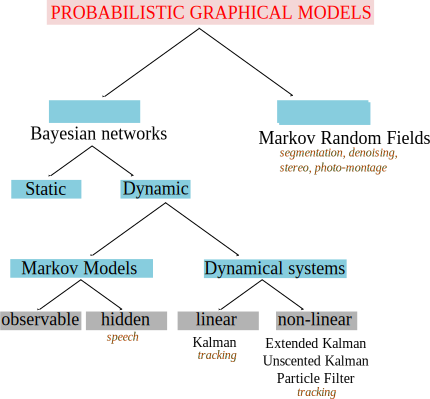
\includegraphics[width=0.9\textwidth]{figs/PRML_PGM_overview.pdf}
	\end{figure}
\end{frame}





\begin{frame}
\frametitle{Tracking}
\framesubtitle{relationship with HMM}
\logoCSIPCPL\mypagenum
	\begin{figure}
		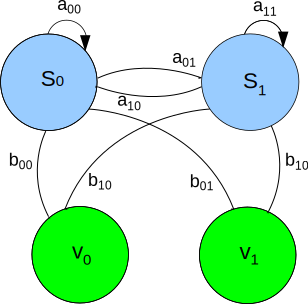
\includegraphics[height=0.3\textheight]{figs/HMM_flowDiagram.pdf}
	\end{figure}
	\begin{figure}
		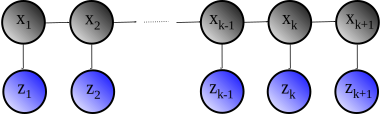
\includegraphics[width=1.0\textwidth]{figs/HMM_flowDiagram2.pdf}
	\end{figure}
\end{frame}



\begin{frame}
\frametitle{Tracking}
\framesubtitle{update}
\logoCSIPCPL\mypagenum
	\begin{figure}
		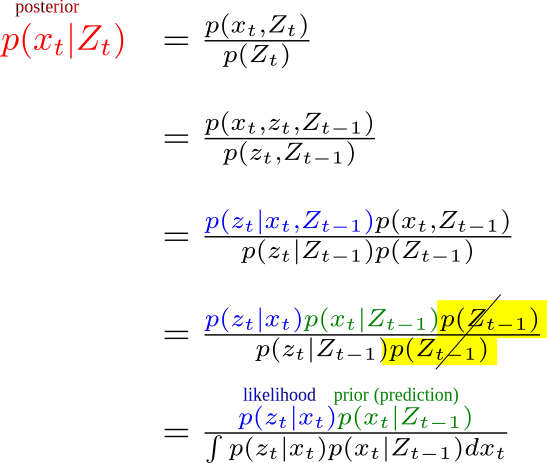
\includegraphics[width=1.0\textwidth]{figs/TRK_EQN_update.pdf}
	\end{figure}
\end{frame}



\begin{frame}
\frametitle{Tracking}
\framesubtitle{prediction}
\logoCSIPCPL\mypagenum
	Chapman Kolmogorov equation
	\begin{figure}
		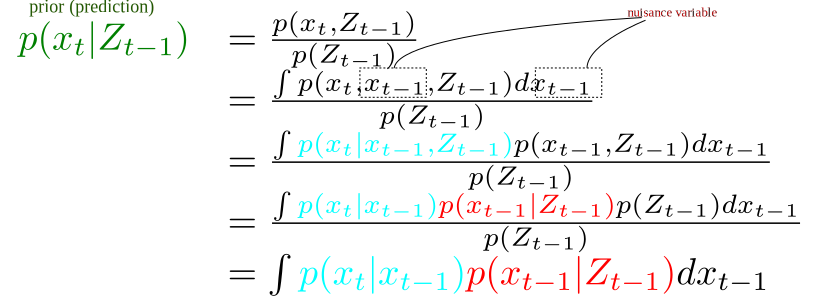
\includegraphics[width=1.0\textwidth]{figs/TRK_EQN_prediction.pdf}
	\end{figure}
\end{frame}

%#######################################################################
\section{Clutter free tracking}
%#######################################################################
%===================================================
\subsection{\ \ \ \ Linear}
%===================================================


%------------------------------------------------
\subsubsection{\ \ \ \ \ \ \ \ Kalman filter}
%------------------------------------------------
\begin{frame}
\frametitle{Kalman Filter}
\framesubtitle{block diagram}
\logoCSIPCPL\mypagenum
	\begin{figure}
		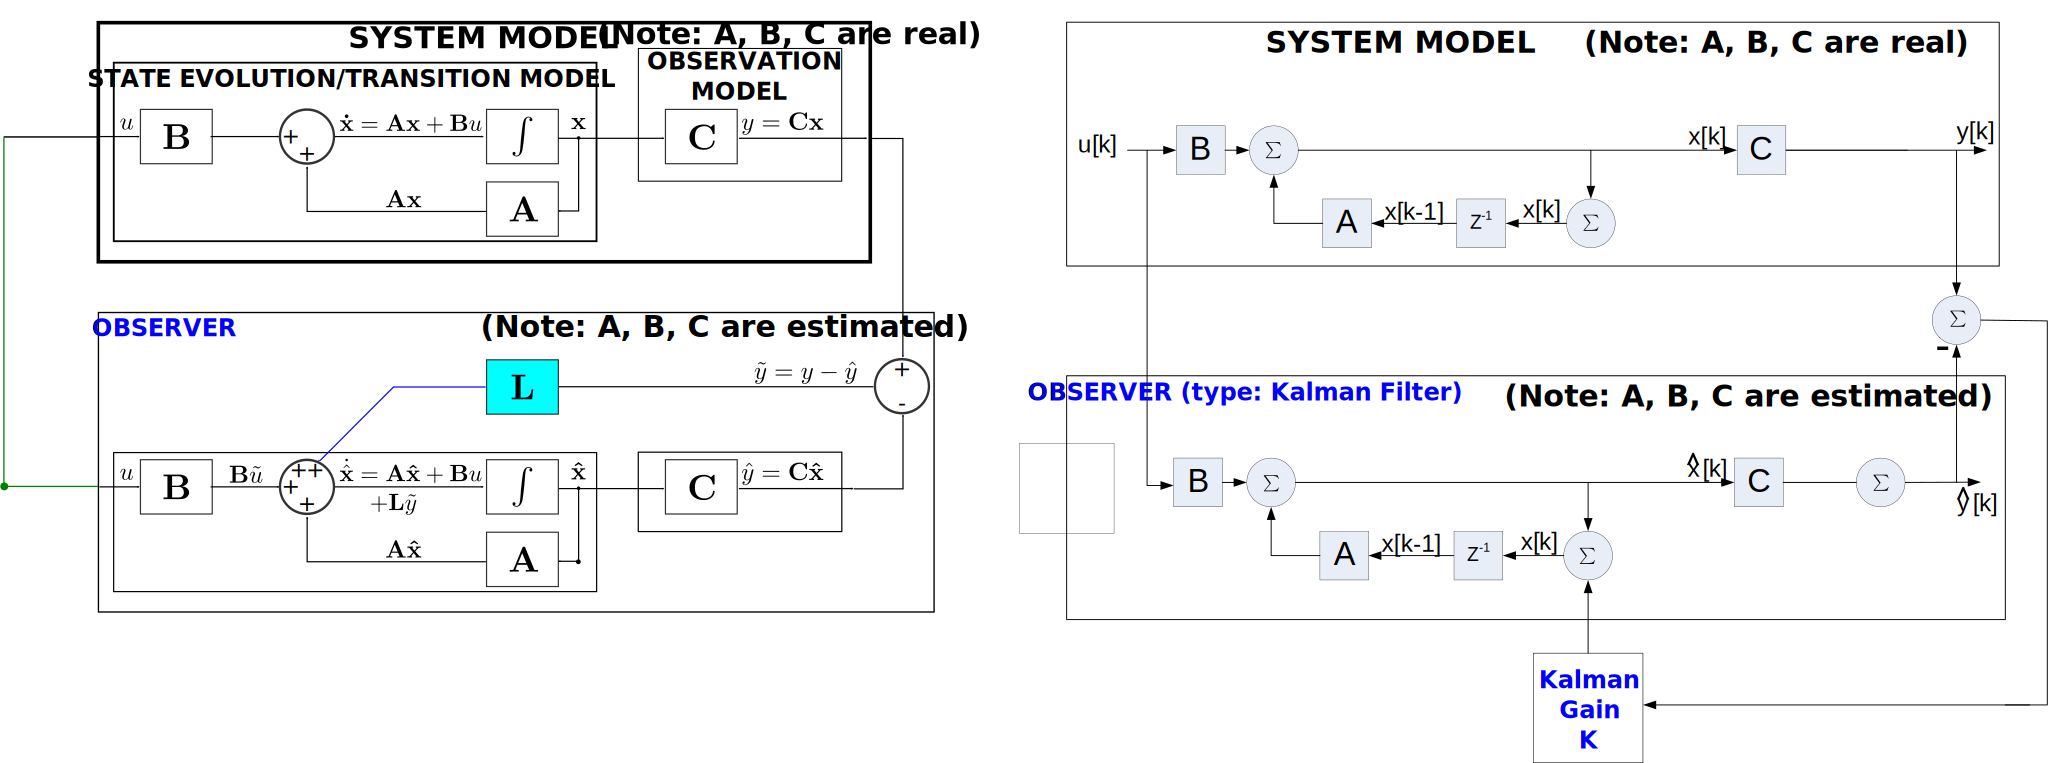
\includegraphics[width=1.0\textwidth]{figs/TRK_KalmanFilter_blockDiagram.pdf}
	\end{figure}
\end{frame}



\begin{frame}
\frametitle{Kalman Filter}
\framesubtitle{overview}
\logoCSIPCPL\mypagenum
	\begin{itemize}
		\item {\color{red}Prior}
			\begin{itemize}
				\item Past information through time $k-1$
				\item summarized approximately by a sufficient statistic in the form of a Gaussian posterior
			\end{itemize}
		\begin{equation*}
			p(x_{k-1|k-1}|Z_{k-1})=\mathcal{N}  (\hat{x}_{k-1|k-1}, P_{k-1|k-1})
		\end{equation*}
		\item {\color{red}Prediction}
			\begin{itemize}  
				\item The state prediction is distributed as,
				\begin{equation*}
					p(x_{k|k-1}|Z_{k-1})=\mathcal{N}  (\hat{x}_{k|k-1}, P_{k|k-1})
				\end{equation*}
				\item The observation prediction is distributed as,
				\begin{equation*}
					p(z_{k|k-1})=\mathcal{N}  (\hat{z}_{k|k-1}, S_k)
				\end{equation*}
			\end{itemize}
		\item {\color{red}Update}
			\begin{itemize} 
				\item innovation
				\item Kalman gain
				\item aposteriori state estimate and aposteriori covariance estimate
			\end{itemize}
	\end{itemize}
\end{frame}



\begin{frame}
\frametitle{Kalman Filter}
\framesubtitle{equations}
\logoCSIPCPL\mypagenum
	\begin{figure}
		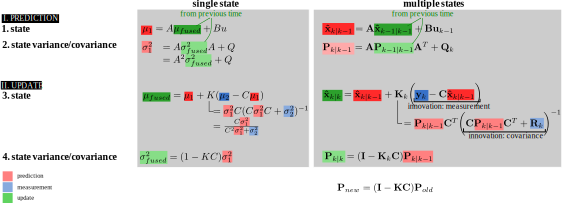
\includegraphics[width=1.0\textwidth]{figs/TRK_KalmanFilter_equations.pdf}
	\end{figure}
\end{frame}

%===================================================
\subsection{\ \ \ \ Non-linear}
%===================================================

%------------------------------------------------
\subsubsection{\ \ \ \ \ \ \ \ Particle filter}
%------------------------------------------------
\begin{frame}
\frametitle{Particle Filter}
\framesubtitle{multi-modal PDF}
\logoCSIPCPL\mypagenum
	\begin{figure}
		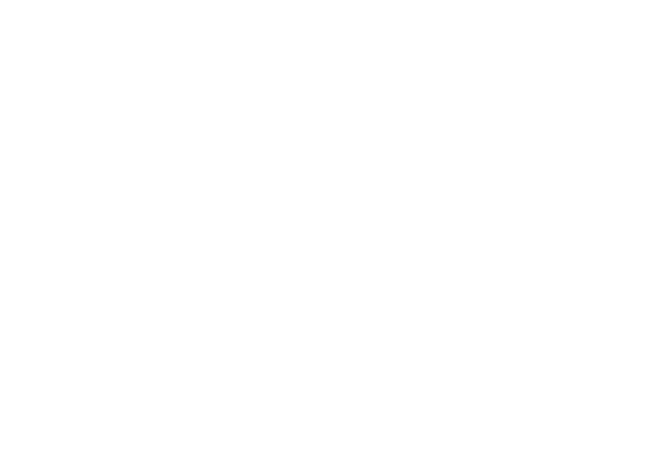
\includegraphics[width=1.0\textwidth]{figs/TRK_ParticleFilter_multimodalPDF.pdf}
	\end{figure}	
\end{frame}




\begin{frame}
\frametitle{Particle Filter}
\framesubtitle{weight update}
\logoCSIPCPL\mypagenum
	\begin{figure}
		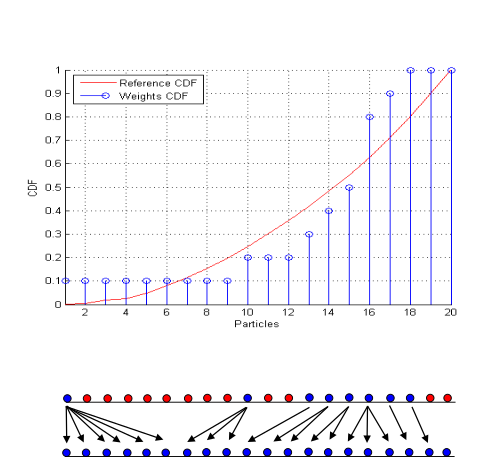
\includegraphics[width=0.9\textwidth]{figs/TRK_ParticleFilter_weightUpdates.pdf}
	\end{figure}	
\end{frame}


%#######################################################################
\section{Tracking in clutter}
%#######################################################################

%===================================================
\subsection{\ \ \ \ Linear}
%===================================================

%\begin{frame}\frametitle{Theory}\logoCSIPCPL\mypagenum
%	\begin{figure}
%		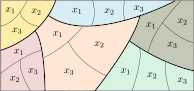
\includegraphics[width=0.7\textwidth]{figs/TRK_PDAF_probability_space.pdf}
%	\end{figure}
%\end{frame}
%---------------------------------------------------------------
\subsubsection{\ \ \ \ \ \ \ \ theory}
%---------------------------------------------------------------
\begin{frame}
\frametitle{Tracking in clutter}
\frametitle{MMSE, MMSE-MAP, MMSE-ML}
\logoCSIPCPL\mypagenum
	\begin{figure}
		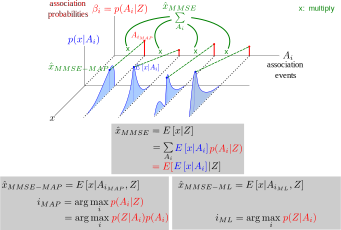
\includegraphics[width=1.0\textwidth]{figs/TRK_clutter_all.pdf}
	\end{figure}
\end{frame}



\begin{frame}
\frametitle{Tracking in clutter}
\framesubtitle{MMSE}
\logoCSIPCPL\mypagenum
	\begin{figure}
		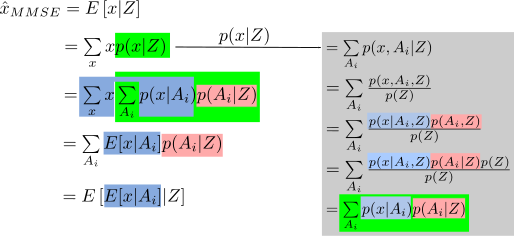
\includegraphics[width=1.0\textwidth]{figs/TRK_clutter_MMSE.pdf}
	\end{figure}
\end{frame}


%---------------------------------------------------------------
\subsubsection{\ \ \ \ \ \ \ \ single target: PDAF}
%---------------------------------------------------------------
\begin{frame}
\frametitle{PDAF}
\framesubtitle{Introduction}
\logoCSIPCPL\mypagenum
	{\color{red} Probabilistic Data Association Filter}
	\begin{itemize}
		\item Computationally efficient 
		\item Data association
		\item Single targets in clutter, high false alarm rate
		\item Extension of Kalman filter
		\begin{itemize}
			\item Primary difference: computation of innovations
			\item Calculates association probabilities to the target for each validated measurement
		\end{itemize}
	\end{itemize}
\end{frame}



%\begin{frame}\frametitle{Other solutions}\logoCSIPCPL\mypagenum
%	\begin{itemize}
%		\item Standard filter: pick one of them, e.g. nearest neighbor (possibly incorrect)
%		\item Track split: one track for every possible measurement (computationally expensive)
%	\end{itemize}
%\end{frame}




\begin{frame}
\frametitle{PDAF}
\framesubtitle{assumptions}
\logoCSIPCPL\mypagenum
	\begin{enumerate}
		\item  {\color{red}{Number of targets}}
		\begin{itemize}
			\item Single target tracking
		\end{itemize}
		\item {\color{red}{False alarms}}
		\begin{itemize} 
			\item At most, one of the validated measurements can be target originated	
			\item Remaining measurements
			\begin{itemize}
				\item incorrect, i.e., false alarms
				\item i.i.d
				\item parametric form: Poisson distribution with known spatial density $\lambda$
				\item non-parametric form: uniform spatial distribution
			\end{itemize}
		\end{itemize}
	\end{enumerate}
\end{frame}
	



\begin{frame}
\frametitle{PDAF}
\framesubtitle{assumptions (cont.)}
\logoCSIPCPL\mypagenum
	\begin{enumerate}\setcounter{enumi}{2}
		\item {\color{red}{Target detection}}
		\begin{itemize} 
			\item Known probability, $P_D$
		\end{itemize}
		%\item Innovation of correct return normally distributed
		\item {\color{red}{Prior}}
		\begin{itemize} 
			\item Density of the state conditioned on the past observations is a Gaussian distribution,		
		\end{itemize}
		\begin{equation*}
			p(\mathbf{x}_{k-1}|Z^{k-1}) = \mathcal{N}  (  \hat{\mathbf{x}}_{k-1|k-1}, \mathbf{P}_{k-1|k-1})
		\end{equation*}
	\end{enumerate}
\end{frame}



\begin{frame}[plain]
\frametitle{PDAF}
\framesubtitle{summary\footnote{Bar-shalom, 2009}}
\logoCSIPCPL\mypagenum
	\begin{changemargin}{-1.3in}{0in}
		\begin{figure}
			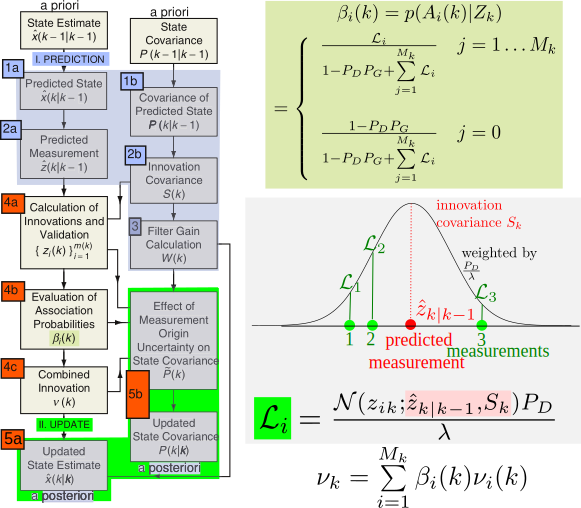
\includegraphics[height=0.8\textheight]{figs/TRK_PDAF_flowDiagram.pdf}
		\end{figure}	
	\end{changemargin}
\end{frame}


\begin{frame}
\frametitle{PDAF}
\framesubtitle{flow diagram, comments}
\logoCSIPCPL\mypagenum
	\begin{itemize} 
		\item for a valid measurement, i.e. $i=1 \ldots M_k$, 
			\begin{itemize}
				\item if $P_D$ is higher, the likelihood $\mathcal{L}_i$ is higher, and so the association probability $\beta_i(k)$ is higher, which makes sense
				\item if $\lambda$ is higher, the poisson distribution is more spread out, and so clutter is more spread out, and so the association probability should be less, which makes sense again
			\end{itemize}
		\item for clutter, i.e. $i=0$
			\begin{itemize}
				\item higher $P_D$ or higher $P_G$ reduces chances of clutter, which is why their product has a negative sign
				\item moreover, the form is such since $\sum \beta_i(k)=1$
			\end{itemize}
	\end{itemize}
\end{frame}





\begin{frame}
\frametitle{PDAF}
\framesubtitle{innovations, step 1}
\logoCSIPCPL\mypagenum
	{\color{red}Measurement validation}
	\begin{itemize} 
		\item only measurements inside a validation gate are accepted. 
		\item $P_G$: If the true measurement is detected,  $P_G$ is the probability that it is in the gate
	\end{itemize}
\end{frame}





\begin{frame}
\frametitle{PDAF}
\framesubtitle{innovations, step 2}
\logoCSIPCPL\mypagenum
	\begin{itemize}
		\item {\color{red} Association events, $A_i$}
		\begin{itemize}
			\item mutually exclusive and exhaustive
			\item Example of three measurements
			\begin{itemize}
				\item $z_1$ originated from target, $z_2$ and $z_3$ are spurious
				\item $z_2$ originated from target, $z_1$ and $z_3$ are spurious
				\item $z_3$ originated from target, $z_1$ and $z_2$ are spurious
				\item All are spurious
			\end{itemize}
		\end{itemize}
		\item {\color{red} Association probabilities, $\beta_i$}
		\begin{itemize}
			\item $\beta_i$ the aposterior probability that the $i$-th return originated from the object in track
			\item$\beta_0$ is the probability that none of the measurements are correct
		\end{itemize}
	\end{itemize}
\end{frame}




\begin{frame}
\frametitle{PDAF}
\framesubtitle{innovations, step 2 (cont.)}
\logoCSIPCPL\mypagenum
	Computing the association probabilities, $\beta_{ik}$,
	\begin{align*}
		\beta_{ik} &\triangleq p(A_{ik}|Z_k)\\
				&=	\left\{ 
						\begin{array}{cc}
							\frac{\mathcal{L}_i}{1-P_DP_G + \sum\limits_{j=1}^{j=M_k} \mathcal{L}_i}  & j=1 \ldots M_k\\ \\
							\frac{1-P_DP_G}{1-P_DP_G + \sum\limits_{j=1}^{j=M_k} \mathcal{L}_i} & j=0
						\end{array} 
					\right. \\
		\mathcal{L}_i&= \frac{\mathcal{N}  (z_{ik};  \hat{z}_{k|k-1}, S_k)P_D}{\lambda}
	\end{align*}
\end{frame}




\begin{frame}
\frametitle{PDAF}
\framesubtitle{innovations, step 2 (cont.)}
\logoCSIPCPL\mypagenum	
	\begin{align*}
		\mathcal{L}_i&= \frac{\mathcal{N}  (z_{ik};  \hat{z}_{k|k-1}, S_k)P_D}{\lambda}
	\end{align*}
	\begin{itemize}
		\item Likelihood $L_i$ is centered around the predicted observation
		\begin{itemize}
			\item Far away clutter has exponentially lower weight
		\end{itemize}
	\end{itemize}
\end{frame}




\begin{frame}
\frametitle{PDAF}
\framesubtitle{innovations, step 3}
\logoCSIPCPL\mypagenum
	{\color{red} Innovations, $\nu_{ik}$}
	\begin{itemize}
		\item $\mathbf{\nu}_{ik}$  for each measurement $\mathbf{z}_{ik}$ are computed using the conditional mean of the observations $\hat{\mathbf{z}}(k|k-1)$:
		\begin{equation*}
			\nu_{ik}  \triangleq \mathbf{z}_{ik} - \hat{\mathbf{z}}(k|k-1) 
		\end{equation*}
	\end{itemize}
\end{frame}



\begin{frame}
\frametitle{PDAF}
\framesubtitle{innovations, step 4}
\logoCSIPCPL\mypagenum
	{\color{red} Combined innovation, $y_k$}
	\begin{itemize}
		\item $\mathbf{\nu}_{ik}$ and $\beta_{ik}$ for each target are combined to form a combined innovation:  
		\begin{equation*}
			y_k  \triangleq \sum_{i=1}^{M_k} \beta_{ik}\nu_{ik}
		\end{equation*}
	\item If there is only one measurement, i.e., $M_k=1$, PDAF becomes equivalent to the Kalman Filter
	\end{itemize}
\end{frame}




\begin{frame}
\frametitle{PDAF}
\framesubtitle{covariance update}
\logoCSIPCPL\mypagenum
	\begin{align*}
		\mathbf{P}_{k|k-1} =
		&\beta_{0k}\mathbf{P}_{k|k-1} +\\
		&\left[1-\beta_{0k}\right]\left[\mathbf{P}_{k|k-1}-\mathbf{K}_k\mathbf{S}_k\mathbf{K}_k'\right] +\\
		&\mathbf{K}_k\left[\sum\limits_{i=1}^{m_k}\beta_{ik}y_{ik}y_{ik}'-y_{k}y_{k}'\right]\mathbf{K}_k' 
	\end{align*}
\end{frame}




\begin{frame}
\frametitle{PDAF}
\framesubtitle{limitations}
\logoCSIPCPL\mypagenum
	\begin{itemize}
		\item The PDAF algorithm makes an assumption that a single target is being tracked.  
		\item Additional targets handled with multiple copies of the filter.  
		\item However, in such cases, measurements from interfering targets do not behave like a Poisson process.  
		\item Solution: JPDAF
	\end{itemize}
\end{frame}



\begin{frame}
\frametitle{PDAF}
\framesubtitle{usage}
\logoCSIPCPL\mypagenum
	PDAF + multiple model Kalman Filters\footnote{Bar-Shalom et al., 2009}:
	\begin{figure}
		\includegraphics[width=0.8\textwidth]{figs/TRK_PDAF_example_US_Navy_ROTHR.jpg}
		\caption {US Navy ROHR (Relocatable Over the Horizon Radar) for long-range surveillance for drug interdiction against aircraft and ships}
	\end{figure}
\end{frame}

%------------------------------------------------------------------
\subsubsection{\ \ \ \ \ \ \ \ multi-target: JPDAF}
%------------------------------------------------------------------

\begin{frame}
\frametitle{JPDAF}
\framesubtitle{Introduction}
\logoCSIPCPL\mypagenum
	{\color{red} Joint Probabilistic Data Association Filter}
	\begin{itemize}
		\item Extension of PDAF to multi-target tracking	
			\begin{itemize}
				\item Only difference: computation of association probabilities, $\beta_{ik}$
			\end{itemize}
		\item Handles multiple targets by considering all measurements for all targets.  
		\item Probability density of each candidate measurement
			\begin{itemize}
				\item Based on all close-by targets
			\end{itemize}
	\end{itemize}
\end{frame}


\begin{frame}
\frametitle{JPDAF}
\framesubtitle{}
\logoCSIPCPL\mypagenum
	\begin{itemize}
		\item $\Omega$: the situation as it is, no processing, just look at validation gates and see which measurements can be associated with which targets, and create a matrix out of this
		\item Joint event $\chi$
			\begin{itemize}
				\item take a target, associate it with all measurements, that's a joint event
			\end{itemize}
		\item Feasible event
			\begin{itemize}
				\item If for a joint event, only one measurement is associated with a target, then the joint event is also a feasible event
				\item take the $\Omega$ matrix, enumerate all possible feasible events
			\end{itemize}
		\item $\tau(j)=1$, the $j$-th observation is not clutter
		\item $\delta(t)=1$, the $t$-th target is associated with some measurement

	\end{itemize}
\end{frame}






\begin{frame}
\frametitle{JPDAF}
\framesubtitle{summary}
\logoCSIPCPL\mypagenum
	\begin{figure}
		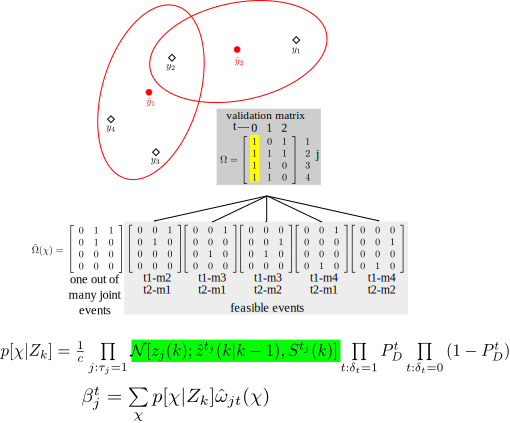
\includegraphics[width=1.0\textwidth]{figs/TRK_JPDAF_twoTargetScenario.pdf}
	\end{figure}
\end{frame}

%\begin{frame}\frametitle{JPDAF}\logoCSIPCPL\mypagenum
%	\begin{enumerate}
%		\item Measurement validation: The measurements are not gated, and all measurements are considered for every target.
%	\end{enumerate}
%\end{frame}		




\begin{frame}
\frametitle{JPDAF}
\framesubtitle{steps}
\logoCSIPCPL\mypagenum
	\begin{itemize}%\setcounter{enumi}{2}
		\item Joint association probabilities for joint association events
		\item $A_{jt}(k)$ is the event that measurement $j$ at time $k$ originated from target $t$
		\begin{equation*}
			A(k) = \bigcap_j A_{jt}(k)
		\end{equation*}
		\item The probability of $A(k)$ given all measurements $Z_k$ is given by
		\begin{align*}
			\small
			p[A(k)|Z^k] 	&= \frac{1}{c} \prod_j \{ \mathcal{N} [z_j(k); \\ 
						&\hat{z}^{t_j}(k|k-1), S^{t_j}(k)] \}^{\tau_j	}\\
						& \prod_t {P^t_D}^{\delta_t}{(1-P_D)}^{1-\delta_t}
		\end{align*}
	\end{itemize}
\end{frame}





\begin{frame}
\frametitle{JPDAF}
\framesubtitle{steps (cont.)}
\logoCSIPCPL\mypagenum
	\begin{itemize}	
		\item A combined innovation is computed using the joint association probabilities using
		\begin{align*}
			\beta_{j}(k) &\triangleq p[A_{jt}(k)|Z_k]  \notag\\
			&= \sum_{A:A_{jt} \in A} p[A(k)|Z_k]
		\end{align*}
	\end{itemize}
\end{frame}




\begin{frame}
\frametitle{JPDAF}
\framesubtitle{usage}
\logoCSIPCPL\mypagenum
	Nearest neighbor JPDAF + EKF\footnote{Bar-Shalom et al., 2009}:
	\begin{columns}
		\begin{column}{1.0in}
			\begin{figure}
			{
				\includegraphics[width=1.0in]{figs/TRK_JPDAF_example_THAAD.jpg}
				\caption {THAAD, \\Theater High Altitude Area Defense)}
			}
			\end{figure}
		\end{column}
		\begin{column}{1.0in}
			\begin{figure}
			{
				\includegraphics[width=1.0in]{figs/TRK_JPDAF_example_Cobra.jpg}
				\caption {Cobra Dane,\\long-range surveillance against ICBMs}
			}
			\end{figure}
		\end{column}
		\begin{column}{1.0in}
			\begin{figure}
			{
				\includegraphics[width=1.0in]{figs/TRK_JPDAF_example_SBX.jpg}
				\caption {SBX,\\long-range surveillance against ICBMs}
			}
			\end{figure}
		\end{column}
	\end{columns}
\end{frame}

%===================================================
\subsection{\ \ \ \ Non-linear}
%===================================================

%--------------------------------------------------------------
\subsubsection{\ \ \ \ \ \ \ \ multi-target: MHT}
%--------------------------------------------------------------
\begin{frame}
\frametitle{Multi-hypothesis tracker}
\logoCSIPCPL\mypagenum
	\begin{enumerate}
	\item {\color{red}Clustering}
		\begin{itemize}
			\item A new measurement is associated with a cluster if it falls within the validation region of any target within the cluster
		\end{itemize}
	\item {\color{red}Hypothesis Generation}
		\begin{itemize} 
			\item New hypotheses are generated for the measurements associated with each cluster
			\item The probability of each hypothesis is calculated
			\item Target estimates are then updated
		\end{itemize}
	\item {\color{red}Reduction}
		\begin{itemize}
			\item In this step, hypotheses are combined or eliminated
		\end{itemize}
	\item {\color{red}Simplify hypothesis matrix}
		\begin{itemize}
			\item Targets that are uniquely associated are removed from the hypothesis matrix
		\end{itemize}
	\end{enumerate}
\end{frame}




\begin{frame}
\frametitle{MHT}
\framesubtitle{usage}
\logoCSIPCPL\mypagenum
	MHT + EKF\footnote{Bar-Shalom et al., 2009}:
	\begin{figure}
		\includegraphics[width=0.7\textwidth]{figs/TRK_MHT_example_UEWR.jpg}
		\caption {UEWR, Upgraded Early Warning Radar, long-range surveillance against ICBMs}
	\end{figure}
\end{frame}


%####################################################################################################
%####################################################################################################
%\bibliographystyle{ieee}
%\bibliography{c:/salman/work/writing/MyCitations}
\end{document}
%####################################################################################################

%####################################################################################################




